\documentclass[leqno]{beamer}
\usepackage[spanish,activeacute]{babel}
\usepackage[utf8]{inputenc}
\usepackage{amsfonts}
\usepackage{enumerate}
\usepackage{amsthm}
\usepackage{graphicx}

\usetheme{CambridgeUS}
\usecolortheme{spruce}

\title{Pr\'actica 1}
\subtitle{Kinect 360}
\author{Anabel G\'omez R\'ios, Jacinto Carrasco Castillo}

\begin{document}

\begin{frame}
\titlepage
\end{frame}

\begin{frame}
\frametitle{Descripción del problema que se aborda}

\begin{itemize}
\item Reconocimiento del esqueleto
\item Reconocimiento de movimientos y gestos
\item Medición del usuario
\item Salida por pantalla para colocar al usuario
\item Interacción del usuario con la aplicación
\end{itemize}
\end{frame}

\begin{frame}
\frametitle{Descripción de la solución que se aporta}

Partimos del proyecto \texttt{Skeleton Basics} perteneciente a Kinect Toolkit. Utilizamos la librería \texttt{Microsoft.Kinect} y creamos una clase \texttt{Gesture} para reconocer las posiciones a realizar por el usuario.\\
\textit{ }\\
Situamos al usuario a una distancia a la que sean visibles la cabeza, el torso y los brazos mediante una línea dibujada en pantalla y mensajes.\\
\textit{ }\\
Indicamos al usuario una posición con los brazos en cruz y lo guiamos mediante marcas dibujadas en pantalla para medirlo.
\end{frame}

\begin{frame}
\frametitle{Descripción de la solución que se aporta}

Con imágenes y marcas en la pantalla, pedimos al usuario que se coloque en la posición inicial, usando las medidas tomadas para determinar la posición.\\
\textit{ }\\
Cuando el usuario mantiene esta posición por dos segundos, se pasa a hacer el movimiento, mostrando con una imagen y por marcas cada una de las tres posiciones que componen el movimiento.
\end{frame}

\begin{frame}
\frametitle{Descripción de la solución que se aporta}

\begin{block}{Código de colores para indicar la corrección de la posición}
\begin{itemize} 
\item Rojo: La parte del cuerpo que se debe situar en la posición está lejos.
\item Amarillo: La parte del cuerpo está cerca.
\item Verde: La parte del cuerpo que se debe situar está en la posición.
\item Verde claro: La parte del cuerpo que se debe situar está en la posición y ha transcurrido más de la mitad del tiempo fijado.
\end{itemize}
\end{block}
\textit{ }\\
Para el botón de salida estos colores se cambian respectivamente por gris, azul, morado y rojo.
\end{frame}

\begin{frame}
\frametitle{Descripción de la solución que se aporta}

Si Kinect no detecta a una persona en algún momento de la ejecución, a la siguiente persona que detecta la vuelve a medir.\\
\textit{ }\\
De esta forma, los círculos que se muestran por pantalla se adaptan al nuevo usuario y éste puede realizar sin problema los movimientos.
\end{frame}

\begin{frame}
\frametitle{Funcionalidades más importantes de \texttt{Gesture}}

\begin{itemize}
\item Proyectar un punto del esqueleto en la pantalla.
\item Dos constructores dependiendo de si el gesto debe comprobar la posición de un punto del esqueleto o de varios.
\item Cambio de color de los objetos en función de la distancia del punto del esqueleto a la posición final.
\item Información de si el gesto ha sido completado (controlar el tiempo que lleva en la posición correcta).
\item Dibujar las posiciones finales mediante círculos.
\item Dibujar la cruz para salir de la aplicación.
\item Reajustar posiciones en caso de que se haya medido mal al usuario.
\end{itemize}
\end{frame}

\begin{frame}
\frametitle{Funcionalidades más importantes de \texttt{MainWindow}}

\begin{itemize}
\item Crear los gestos a reconocer.
\item Controlar qué gesto y acciones se deben llevar a cabo mediante un conjunto de estados.
\item Medir al usuario.
\item Mostrar las imágenes de los gestos.
\item Mostrar los mensajes.
\item Controlar si se están detectando usuarios.
\end{itemize}
\end{frame}

\begin{frame}
\frametitle{Errores frecuentes}

\begin{itemize}
\item Skeletons detectados que no se corresponden con los humanos en movimiento seguidos.
\item Superponer la imagen de vídeo con los dibujos necesarios para situar al esqueleto.
\item Generar la ruta de las imágenes para mostrarlas por pantalla.
\item Falta de precisión de Kinect.
\end{itemize}
\end{frame}


%\begin{frame}
%\frametitle{Bonus: FAQ}
%\begin{figure}[htb]
%\centering
%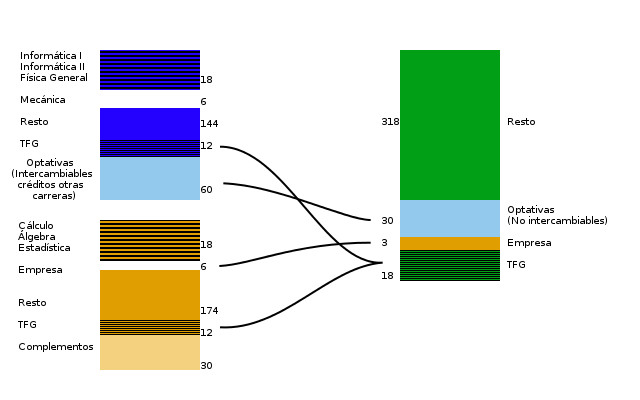
\includegraphics[width=\textwidth]{creditos}
%\end{figure}
%\end{frame}

\end{document}
